\documentclass[sigconf,anonymous,review]{acmart}

\usepackage[ruled, vlined, linesnumbered]{algorithm2e}
\usepackage[toc,page]{appendix}

\usepackage{bm}
\usepackage{pifont}

\newtheorem{definition}{Definition}
\newtheorem{theorem}{Theorem}
\newtheorem{lemma}{Lemma}
\newtheorem{corollary}{Corollary}

\graphicspath{{figs/}}
\usepackage{booktabs}
\usepackage{multirow}
% \newcommand{\tabincell}[2]{\begin{tabular}{@{}#1@{}}#2\end{tabular}}

\usepackage{wrapfig}

\definecolor{green}{rgb}{0.0, 0.55, 0.13}

\title{Taming the Performance Unpredictability of the Maximum $k$-Plex Finding Algorithms by Machine Learning}

\begin{document}

\begin{abstract}
A $k$-plex is a dense structure where every vertex can be disconnected with at most $k$ vertices. Finding a maximum $k$-plex (M$k$P) in a big graph is important in many real applications such as community detection and biological network analysis. Numerous M$k$P algorithms have emerged in recent years featuring a broad range of sophisticated pruning techniques that fall in three categories, those for (1)~branching, (2)~bounding, and (3)~reduction during subgraph exploration. Two recent winners are (1)~U-M$k$P which features effective branching methods, and (2)~AltRB which features an alternated reduction-and-bound (abbr.\ altRB) method, both significantly beating prior works but have not been compared with each other. 

In this paper, we explore how to combine U-M$k$P's branching technique with the altRB method to achieve the best performance. U-M$k$P adopts a sparse data representation that favors buffer reuse during backtracking, while AltRB adopts a dense bit encoding representation that favors set operations. There is no clear winner of the data representations so we implement both versions, and they can enable U-M$k$P's branching technique and the altRB method, giving five algorithm variants. However, the running time of some variants can be orders of magnitude faster than others, but there is no clear winner or loser among these variants and the result vary case by case in terms of the graph and the value of $k$ and is highly unpredictable. We, therefore, explore the use of machine learning to predict the fastest algorithm based on the graph features after an initial reduction pruning as well as the value of $k$, and extensive experiments show that {\color{red} ...... statement on accuracy based on Naman's results: which models are the best? which models are complementary to each other? ensemble can reach 0 failure?  ... Our source code is released at \url{https://???}.}
\end{abstract}
\maketitle

\vspace{-1mm}
\section{Introduction}\label{sec:intro}
Finding cohesive subgraphs in a large graph is useful in applications such as finding protein complexes or biologically relevant functional groups~\cite{bader2003automated,bu2003topological,hu2005mining,ucar2006improving} and social communities~\cite{li2014uncovering,hopcroft2004tracking}. Clique is a classic notion of cohesive subgraph where every pair of vertices are connected by an edge (see Figure~\ref{fig:ex2plex}(a)). However, communities rarely appear in the form of cliques in real graphs due to various reasons such as the existence of data noise~\cite{pattillo2013clique,www22maximal,d2k,kdd17}. 
%
As a relaxed clique model, $k$-plex~\cite{seidman1978graph} is defined as a graph where every vertex $v$ is adjacent to all but at most $k$ vertices (including $v$ itself). Figure~\ref{fig:ex2plex}(b) shows a 2-plex where every vertex is not adjacent to at most $k=2$ vertices. For example, $a$ is not connected to $\{a, c\}$ (see dotted edges in Figure~\ref{fig:ex2plex}(c)). 
%
It has found extensive applications in the analysis of social networks~\cite{seidman1978graph}, especially in the community detection~\cite{pattillo2013clique,d2k}. However, mining $k$-plex structures is NP-hard~\cite{DBLP:journals/jcss/LewisY80,DBLP:journals/ior/BalasundaramBH11}, so existing algorithms rely on branch-and-bound search which runs in exponential time, but utilize effective pruning techniques to make the search process tractable on large graphs.

\begin{figure}[t]
  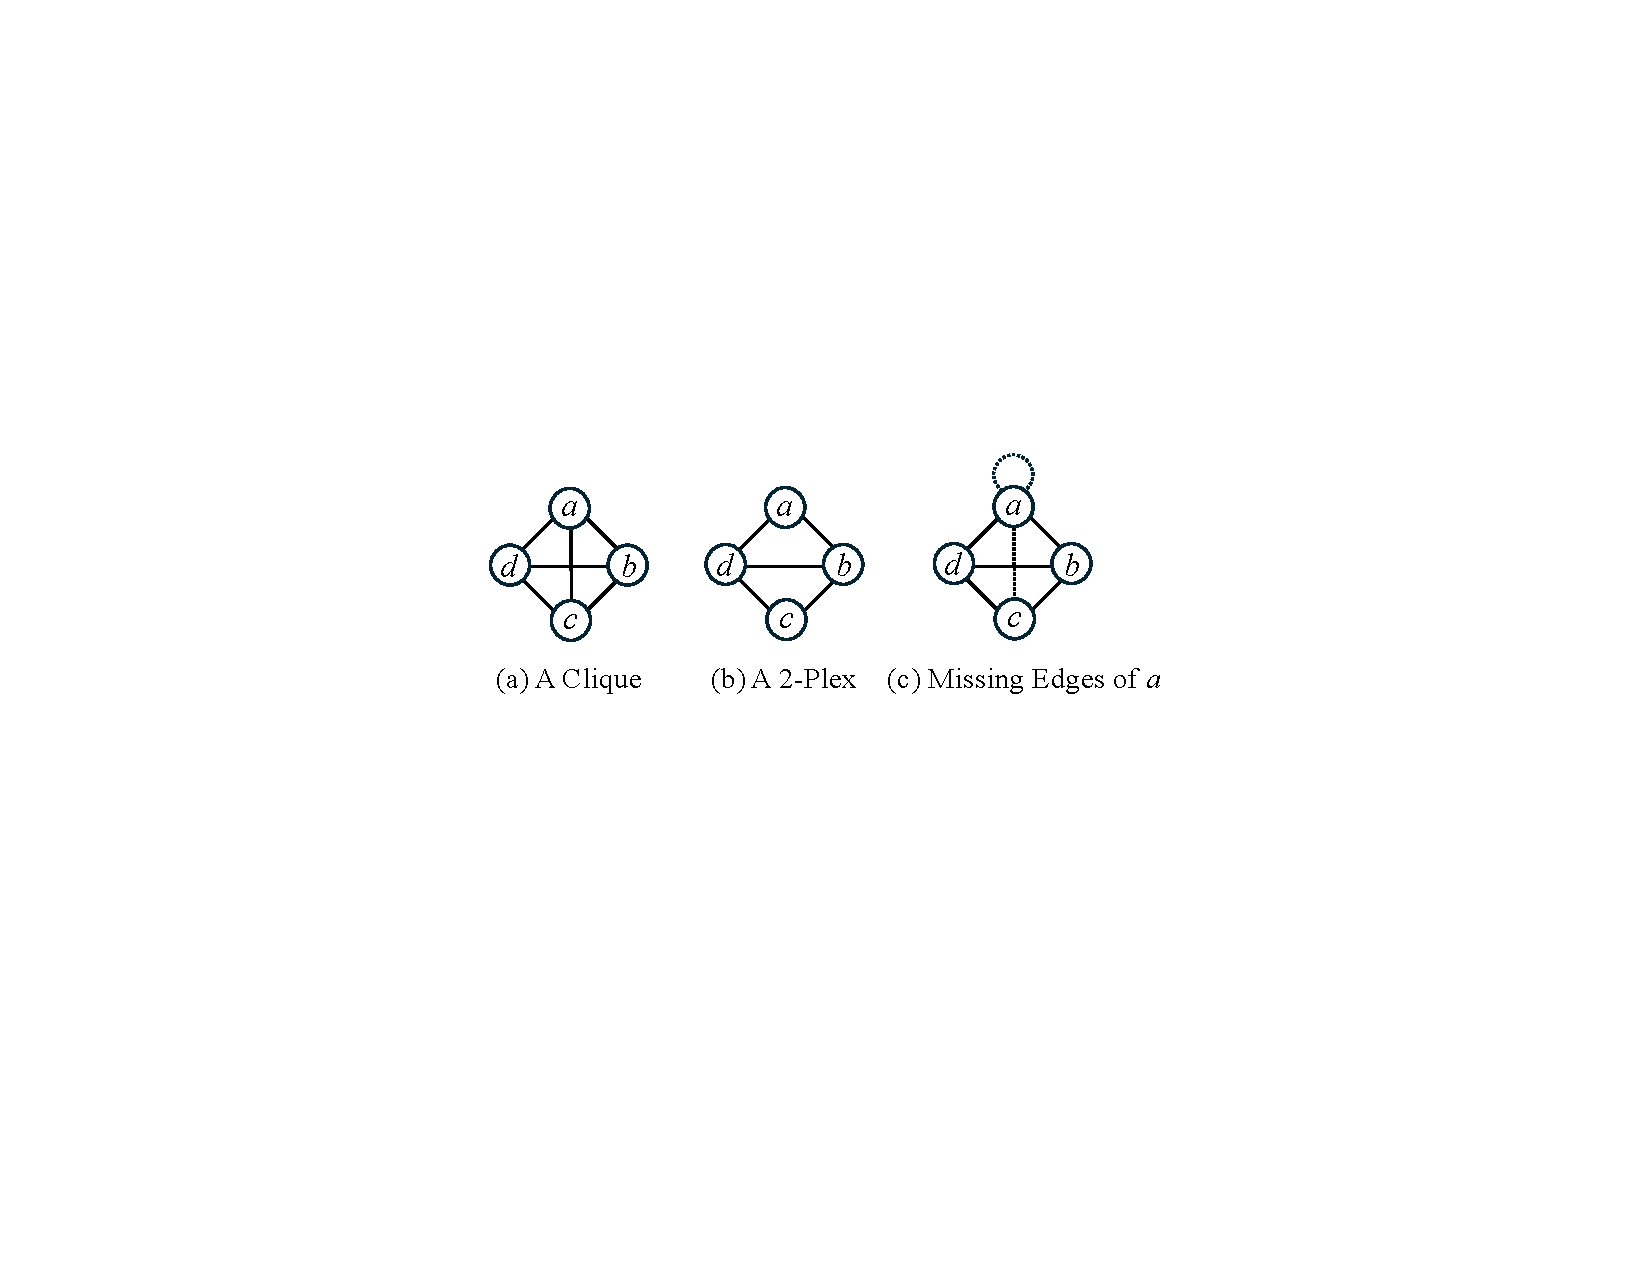
\includegraphics[width=0.7\columnwidth]{ex2plex}
  \vspace{-3mm}
  \caption{Examples of a Clique and a 2-Plex}\label{fig:ex2plex}
  \vspace{-3mm}
\end{figure}

In this paper, we study the problem of finding a maximum $k$-plex (M$k$P), i.e., only one is returned when there are ties. The M$k$P algorithm can be extended to find all M$k$Ps using the method introduced in~\cite{akhlaque_vldb}. In recent years, there is a surge of M$k$P algorithms with new pruning techniques proposed by the DB and AI communities to significantly speed up computation, such as U-M$k$P~\cite{akhlaque_vldb}, AltRB~\cite{clong_vldb}, kPlexT~\cite{kPlexT} Maple~\cite{Maple}, Seesaw~\cite{seesaw}, DiseMKP~\cite{DiseMKP}, kPlexS~\cite{kPlexS}, KpLeX~\cite{KpLeX-MKP}, Maplex~\cite{Maplex}, BnB~\cite{BnB} and BS~\cite{BS}. Figure~\ref{fig:dominance} shows the performance dominance relationships reported by the respective papers to their compared algorithms. Among them, U-M$k$P and AltRB are winners that significantly beat the M$k$P other algorithms, but they have not been compared with each other yet.

\begin{figure}[t]
  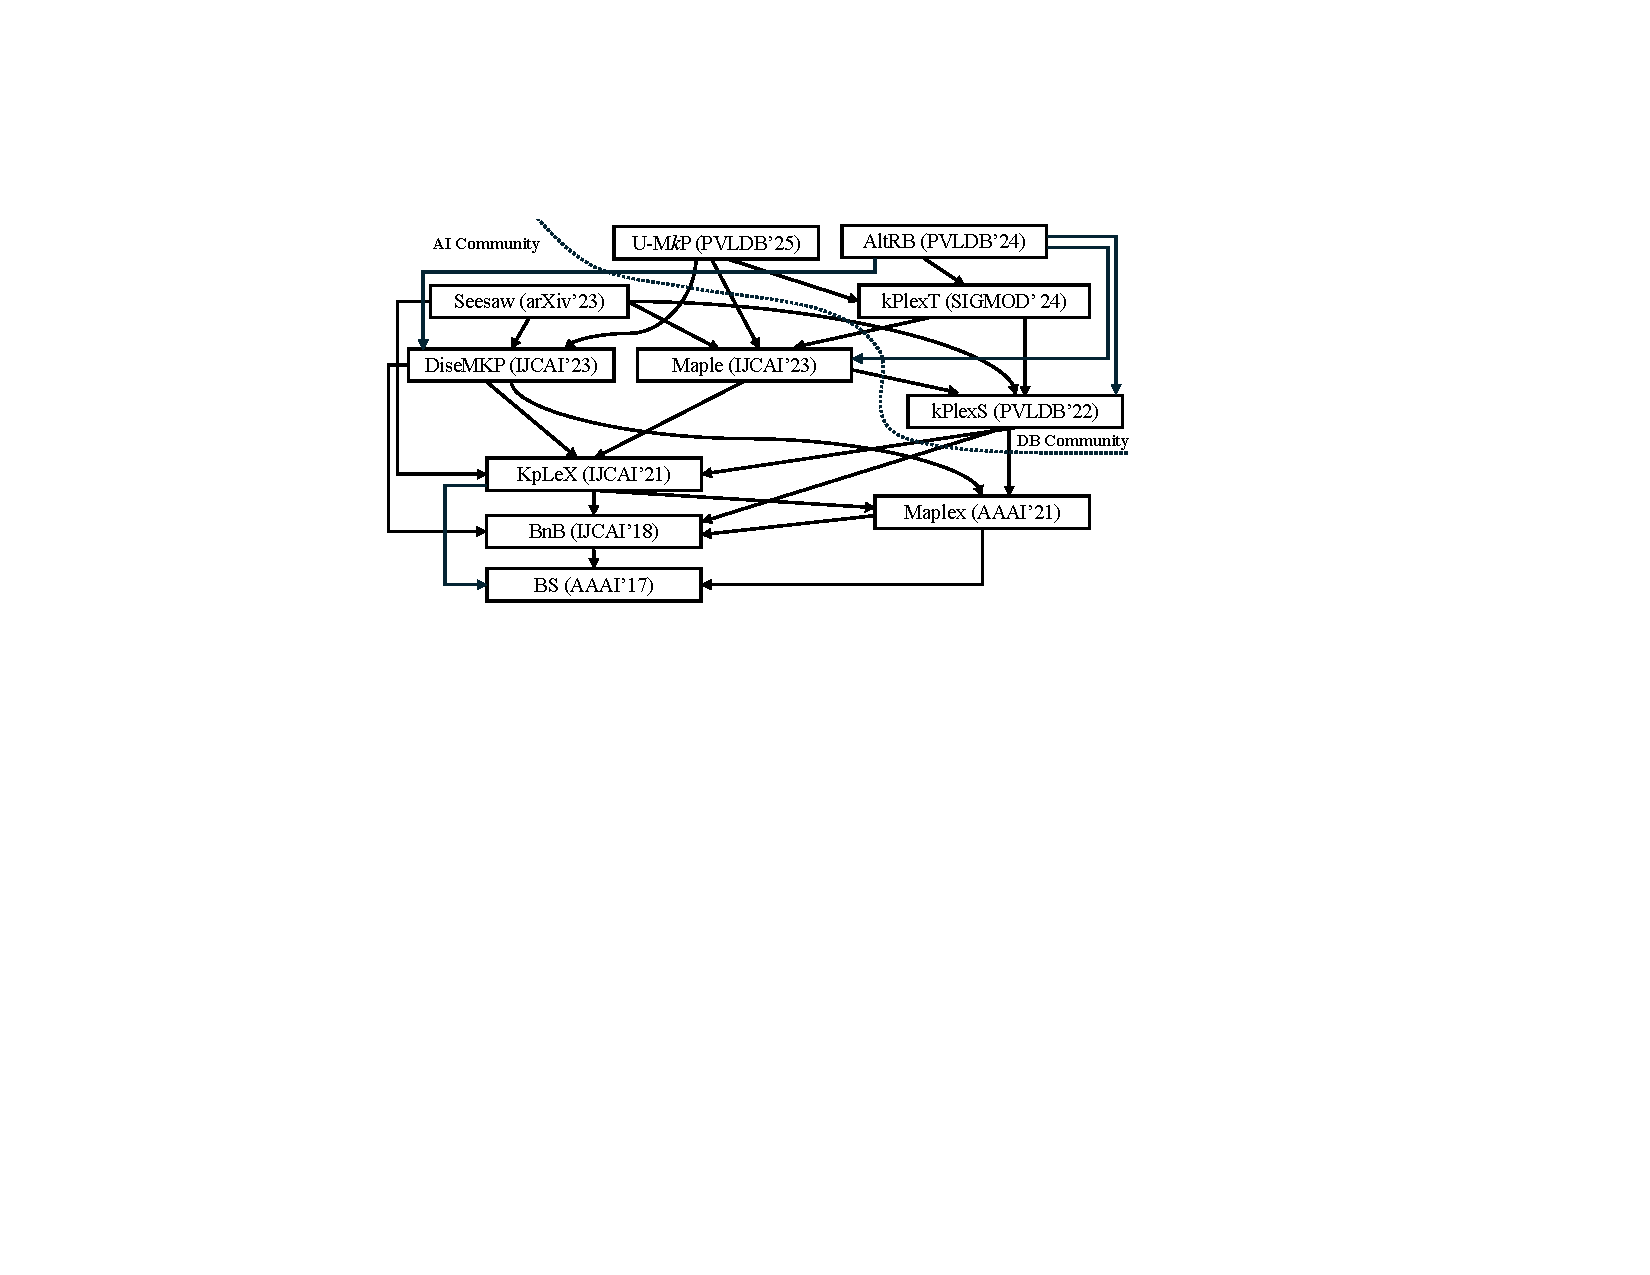
\includegraphics[width=0.86\columnwidth]{dominance}
  \vspace{-3mm}
  \caption{Reported Algorithm Dominance Relationships}\label{fig:dominance}
  \vspace{-5mm}
\end{figure}

Specifically, U-M$k$P~\cite{akhlaque_vldb} is a common framework that unifies the pruning techniques from all the other M$k$P algorithms except for AltRB~\cite{clong_vldb}, which summarizes the techniques into three categories, those for (1)~branching, (2)~upper bounding, and (3)~reduction during subgraph exploration. Through extensive experimental study, a default configuration of the pruning techniques that works generally well has been identified, featuring effective branching methods that depends on the value of $k$: S-based branching method (we will introduce later) is used when $k\leq 5$ and pivot-based method is used when $k>5$. AltRB~\cite{clong_vldb}, on the other hand, features an alternated reduction-and-bound (abbr.\ altRB) method that significantly reduces the search space. A key goal of this work is to combine U-M$k$P's branching techniques with the altRB method to further improve the performance of M$k$P finding.

Interestingly, our analysis reveals that U-M$k$P and AltRB employ distinct data structures for maintaining the explored and candidate vertex sets, exhibiting unique tradeoffs between the {\em ability of incremental updates} and the {\em computational overhead of set operations}. It is difficult to find simple rules to predict which data representation wins a priori, as results vary significantly across different problem instances. 
%
To harness these complementary strengths, we implement: (1) U-M$k$P's two branching techniques within AltRB, and (2) the altRB method within the U-M$k$P framework. Combined with the original U-M$k$P and AltRB, this yields five competitive algorithms for M$k$P finding, providing a portfolio of high-performance candidates to choose from for execution at the runtime.

While certain algorithm variants demonstrate orders-of-magnitu-de % ===== note the line split
speed improvements over others, no single variant consistently outperforms across all scenarios. The relative performance depends intricately on both graph characteristics and the parameter $k$, exhibiting high unpredictability. To address this, we develop a machine learning approach to predict the fastest algorithm using graph features (after initial reduction pruning) and the value of $k$.

This prediction is essentially a five-class classification problem, but requires specialized treatment in the machine learning workflow to optimize algorithm selection. Specifically, in some problem instances, multiple winner candidates demonstrate statistically indistinguishable performance (e.g., $\leq 5\%$ faster or simply a tie), requiring a model to accommodate all optimal algorithm options (rather than to force a single prediction) during training and evaluation. Given a problem instance (i.e., a graph plus a parameter $k$), the focus should be to avoid selecting a poor algorithm option that runs much slower (e.g., by orders of magnitude) than the fastest. 

For training, we consider a {\em time-discrepancy-based sample weighting scheme}, which gives a training sample $\mathbf{x}$ a higher weight $w(\mathbf{x})$ if the running time of different algorithm candidates varies a lot. Note that making the correct prediction for such a sample is crucial since a wrong prediction would lead to a much longer running time, while in contrast, the algorithm selection is not important if all candidates run for more or less the same time. 
%
We also consider a {\em tie-aware weight splitting approach}, where given a training sample $\mathbf{x}$, if $k$ algorithms are all the fastest with a tie {\color{red} (!!! to Naman: not just handling exact ties but also accommodating/tolerating small differences for replicating, e.g., if time gap is within 5\%)}, 
%
then we create $k$ instances of this sample with each instance replicating $\mathbf{x}$'s input features but using a different algorithm label from the $k$ algorithms. Each instance has weight $w(\mathbf{x})/k$ so that the weight of all instances sum up to be $w(\mathbf{x})$. Finally, we adopt {\em (dense) probabilistic categorical cross-entropy loss} for supervision whenever applicable, where ``soft'' probabilistic labels are used so that algorithms with close running times will have similar probabilities of being selected. 
% todo: define $w(\mathbf{x})$

For evaluation, we define metrics such as accuracy, precision and recall to accommodate ties, i.e., a prediction is considered correct as long as any of the fastest algorithms is selected. 
%
{\color{red} (!!! to Naman: to generalize tie to allow 5\% tolerance of time to be considered correct)} 
%
We also define time-based metrics that indicate the relative increase of running time when using the model-predicted algorithm instead of the fastest algorithm (assuming there is an oracle predictor that does not make mistakes). 
%
{\color{red}... say sth about failure cases to visual examination, and ensemble ...}

To curate a dataset for model training and evaluation, we collecte a total of 2741 graphs from three sources: SNAP~\cite{SNAP}, KONECT~\cite{KONECT} and Network Repository~\cite{NetworkRepository}, which include both real and synthetic graphs. As a preprocessing step before subgraph exploration, kPlexS~\cite{kPlexS} proposes to use a heuristic algorithm to find a large $k$-plex $P$ as well as an upper bound $ub$ on the size of any M$k$P in $G$, by running the peeling algorithm in linear time. If $|P|=ub$, then $P$ is already an M$k$P and can be directly returned; otherwise (2)~we can still prune those search branches that cannot lead to a larger $k$-plex with size at least $(|P|+1)$ during subgraph exploration. This preprocessing step is adopted by the latest algorithms including U-M$k$P~\cite{akhlaque_vldb} and AltRB~\cite{clong_vldb}, and this work also adopts it. Among the 2741 graphs, {\color{red} we exclude 2426 graphs since either the fast preprocessing directly finds an M$k$P on them, or all five candidate algorithms run for more than 1800 seconds (which is our timeout threshold to avoid long-running jobs) for all tested values of $k$.} % todo: Akhlaque: 2 separate numbers
%
Among the remaining graphs, an M$k$P can be found on 198 of them in less than a second by all algorithms for all values of $k$, so we also exclude them, leaving only 117 graphs in our curated dataset that are interesting for our machine learning study.

Each combination of dataset and $k$ gives one sample for machine learning, so our dataset is not large and we only consider conventional statistical machine learning models and small neural network models. We remark that our subgraph feature extraction does not incur extra cost since all our graph statistics are straightforward to obtain, including the sizes of $k$-cores which is a byproduct of the preprocessing step that runs the peeling algorithm. Moreover, deploying a trained model for algorithm selection given a new graph takes negligible time since we use small models. 
%
{\color{red}... todo: comment on model performance like in abstract...}

The main contributions of this paper are summarized as follows:
\begin{itemize}
\item We explore the two winner M$k$P algorithms U-M$k$P~\cite{akhlaque_vldb} and AltRB~\cite{clong_vldb}, and propose a unified algorithm framework to combine their pruning techniques. Using this algorithm framework, we screened thousands of public graphs to curate a dataset of graphs interesting for our learning problem.
\item We survey the difference of data structures for vertex sets used by U-M$k$P and AltRB during subgraph exploration and their pros and cons, and propose five competitive algorithm candidates decided by the data structure and adopted pruning techniques for learning-based selection.
\item For machine learning, we propose techniques to put larger weights on samples where the selection decision is critical during training, and techniques to accommodate winning algorithms with ties during both training and evaluation.
\item Extensive experiments are conducted which {\color{red}... todo: comment on model performance like in abstract...}
\end{itemize}

The rest of this paper is summarized as follows. Section~\ref{sec:related} reviews the set enumeration procedure used by M$k$P algorithms, and surveys recent advances in M$k$P techniques. Then, Section~\ref{sec:kplex} presents our unified M$k$P framework, detailing search-space pruning strategies unique to U-M$k$P and AltRB. Section~\ref{sec:set} describes the distinct set representation methods employed by U-M$k$P and AltRB. Section~\ref{sec:learn} presents our five competitive algorithm variants generated by combining different pruning techniques and set representations, and proposes our learning-based algorithm selection method. Finally, Section~\ref{sec:results} reports experiments and Section~\ref{sec:conclude} concludes this paper.

\vspace{-1mm}
\section{Preliminaries and Related Work}\label{sec:related}

\noindent {\bf Notations.} 
We consider an undirected and unweighted simple graph $G=(V, E)$, where $V$ is the vertex set, and $E$ is edge set. The degree of a vertex $v$ is denoted by $d_G(v)=|N_G(v)|$. 
We also define the concept of {\em non-neighbor}: a vertex $u$ is a non-neighbor of $v$ in $G$ if $(u, v)\not\in E$. Accordingly, the set of non-neighbors of $v$ is denoted by $\overline{N_G}(v)=V- N_G(v)$, and we denote its cardinality by $\overline{d_G}(v)=|\overline{N_G}(v)|$.
Given a vertex subset $S\subseteq V$, we denote by $G[S]=(S, E[S])$ the subgraph of $G$ induced by $S$, where $E[S]=\{(u,v)\in E\mid u,v\in S\}$. We simplify the notation $N_{G[S]}(v)$ to $N_S(v)$, and define other notations such as $N_S(v), \overline{N_S}(v)$ and $d_S(v)$ in a similar manner. For an arbitrary graph $g$, $V(g)$ and $E(g)$ denote the vertex set and edge set of $g$, respectively. 
The diameter of $G$, denoted by $\Delta(G)$ is the shortest-path distance of the farthest pair of vertices in $G$, measured by the number of hops.

\vspace{1mm}
\noindent {\bf Problem Definition.} We next define $k$-plex and M$k$P.

\vspace{-1mm}
\begin{definition}(\emph{$k$-Plex})\label{def:kplex}
    A graph $g$ is a $k$-plex if every vertex $v\in V(g)$ has at least $|V(g)|-k$ neighbors in $g$, i.e., $d_g(v)\ge |V(g)|-k$. Equivalently, $g$ is a $k$-plex if every vertex $v\in V(g)$ has at most $k$ non-neighbors in $g$ (including $v$ itself as a non-neighbor), i.e., $\overline{d_g}(v)\le k$.
\end{definition}

\vspace{-2mm}
\begin{definition}(\emph{Maximum $k$-Plex Finding})\label{def:MkP}
  Given a graph $G$, the maximum $k$-plex finding problem finds a largest vertex set $P\subseteq V$ such that the subgraph $G[P]$ induced by $P$ is a $k$-plex. 
\end{definition}
\vspace{-1mm}

\vspace{1mm}
\noindent {\bf Hereditariness and Diameter of $k$-Plex.} 
Note that $k$-plex satisfies the hereditary property which says that: any induced subgraph (denoted by $g'$) of a $k$-plex $g$ is also a $k$-plex, since a vertex in $g'$ cannot miss more neighbors than those already missed in $g$.

Moreover, as proved by~\cite{BS}, the diameter of $k$-plexes with a reasonably large size (which is usually the case for M$k$Ps) is bounded:
\begin{theorem}
\label{lemma::diameter0}
For a $k$-plex $P$ and any integer $c\geq 2$, if $|P|> 2k-c$, then $\Delta(P)\leq c$~\cite{BS}.
\end{theorem}

Most works~\cite{kPlexS,Maple} only consider the case when $c=2$ by assuming $|P|\geq 2k-1$, which gives the following corollary:
\begin{theorem}
\label{lemma::diameter}
    Given a $k$-plex $P$, if  $|P|\geq 2k-1$, then $\Delta(P)\leq 2$.
\end{theorem}

The assumption $|P|\geq 2k-1$ is reasonable for a maximum $k$-plex $P$, %that we target, 
since natural communities that our M$k$P problems aim to discover are connected, and $2k-1$ is relatively small. For example, when $k=5$, we only require $|P|\geq 9$. Note that a $k$-plex with~$|P|=2k-2$ may be disconnected (e.g., formed by two disjoint $(k-1)$-cliques).

\begin{algorithm}[!t]
  \DontPrintSemicolon
  \SetKwBlock{Begin}{function}{end function}
  \Begin($\text{BB\_basic}{(}S, R, g{)}$\ \ \ \ \# The basic $\text{BB}{(}.{)}$ variant){
    {\bf if} (reduce\_and\_prune$(S, R, g)=\textit{true}$) {\bf then\ \ return}\;\label{bb:l1}
    \For{{\em\bf each }$v\in R$}{ \label{bb:l2}
      BB\_basic$(S\cup\{v\}, R-\{v\}, g)$\; \label{bb:l3}
      $R\gets R-\{v\}$\label{bb:l4}
      }
      }
      \caption{Basic Branch-and-Bound Search}    
      \label{algo:BB}
    \end{algorithm}
%\setlength{\textfloatsep}{0pt}

\begin{figure}[t]
\vspace{-3mm}
  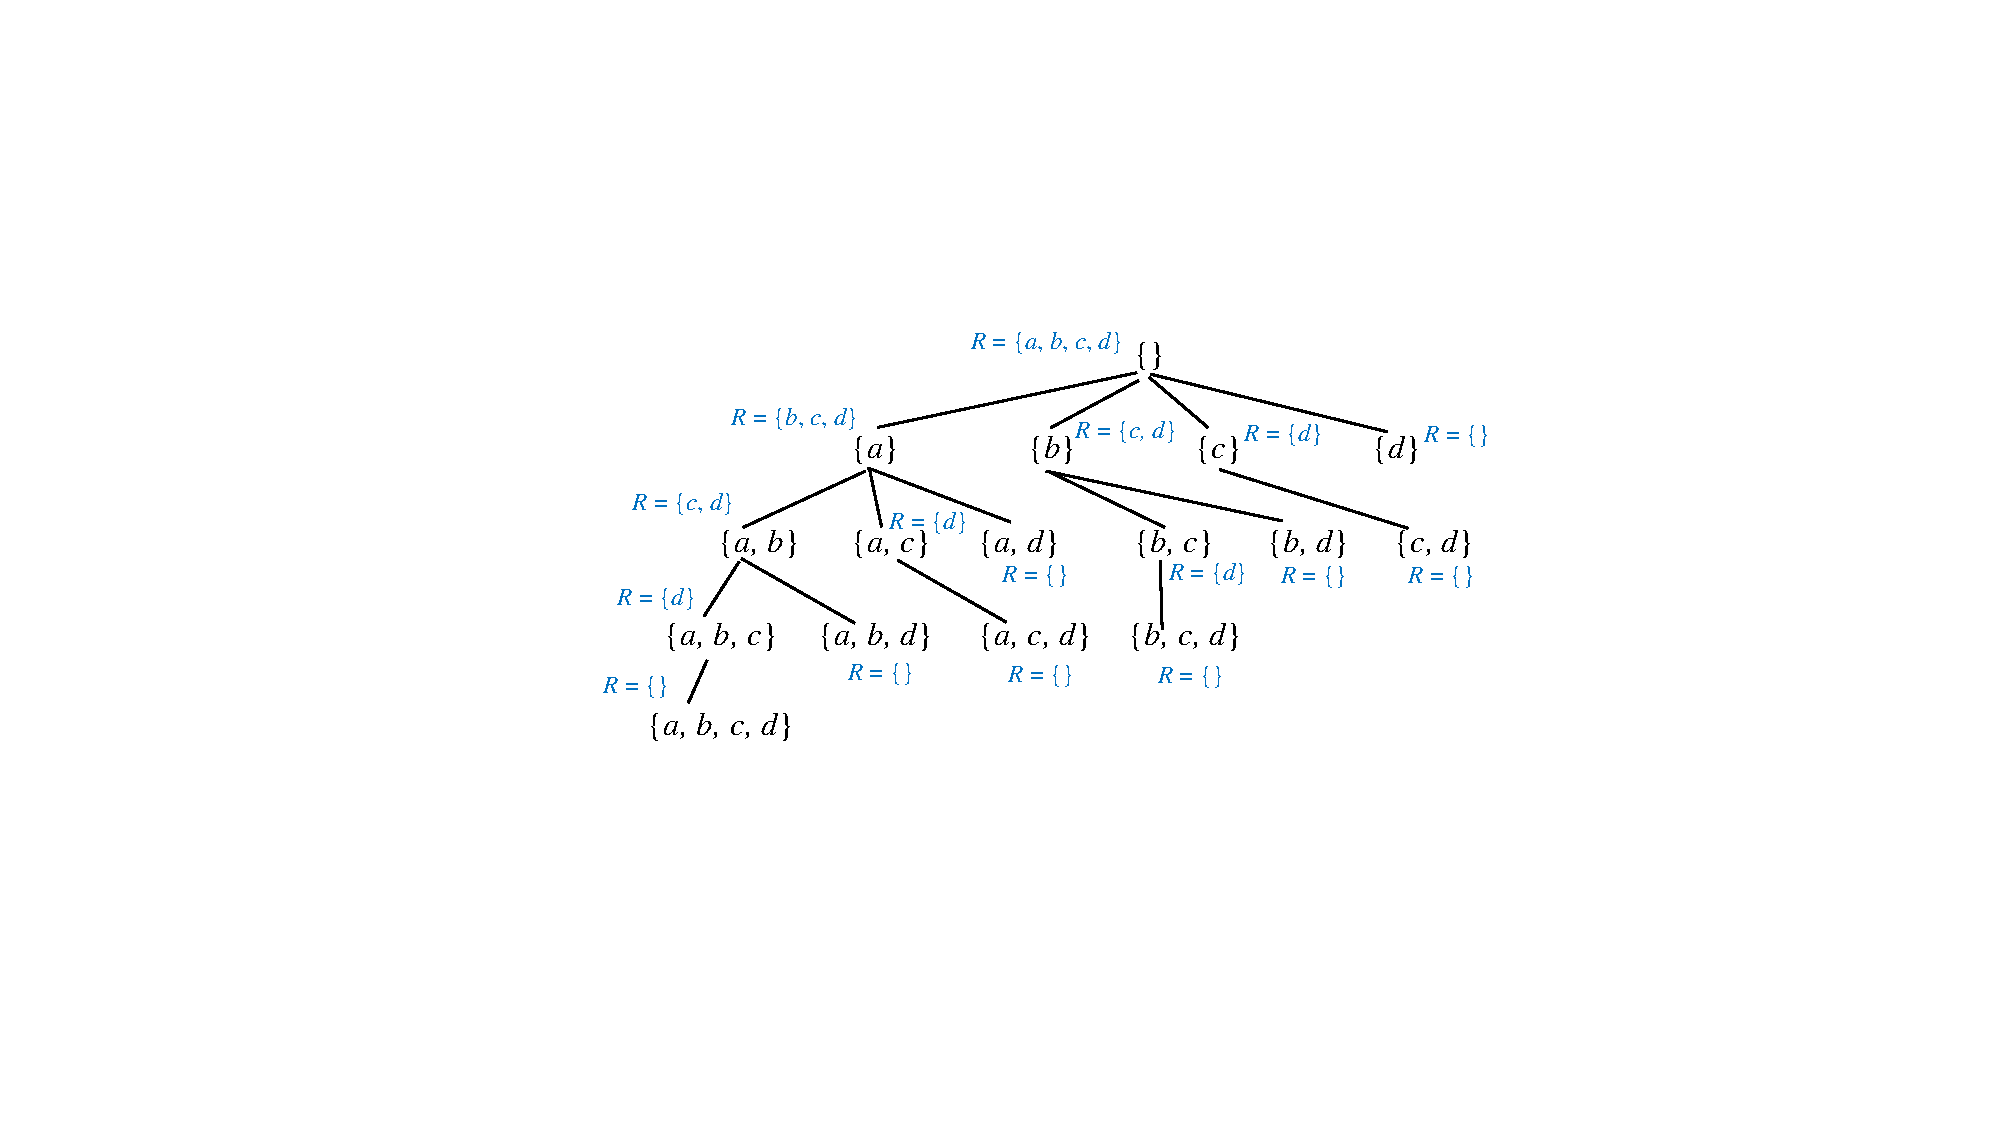
\includegraphics[width=0.9\columnwidth]{set-enum}
  \vspace{-2mm}
  \caption{Set-Enumeration Search Tree}\label{fig:set-enum}
  \vspace{-2mm}
\end{figure}

\vspace{1mm}
\noindent {\bf Subgraph Exploration by Branch and Bound.} 
All existing M$k$P algorithms follow (but are variants of) the branch-and-bound search framework shown in Algorithm~\ref{algo:BB}, where $S$ is the set of vertices already included into the current subgraph, and $R$ is the set of candidate vertices yet to be added to $S$ to form a larger subgraph that can become an M$k$P. 
Specifically, given a vertex-set pair $\langle S, R\rangle$ in graph $g$, Line~2 first calls a function reduce\_and\_prune$(S, R, g)$ to apply reduction and upper-bounding rules, which may decide that the entire search branch to extend $S$ is unpromising so that {\em true} is returned, in which case Line~2 returns directly to terminate the extension of $S$. We will discuss this function in more detail in Section~\ref{sec:kplex}. If the branch is not pruned, Line~3 then takes the next candidate $v\in R$, and split the search space into two cases: (1)~$v$ is in the M$k$P to find, in which case Line~4 further extends $\langle S\cup\{v\}, R-\{v\}\rangle$ by recursion; (2)~$v$ is not in the M$k$P to find, in which case Line~5 removes $v$ so that it will not appear in future iterations of the for-loop in Line~3. 
%
Figure~\ref{fig:set-enum} illustrates the search process of Algorithm~\ref{algo:BB} on a toy graph with four vertices $a$, $b$, $c$ and $d$, which corresponds to a set-enumeration search tree where each node denotes $S$ and we also annotate its corresponding $R$ near the node (assuming that no node is pruned, and that vertices in $R$ are always ordered with $a<b<c<d$). We can see that the search space is perfectly partitioned without redundancy. Note that calling Algorithm~\ref{algo:BB} on $S$ basically grows the set-enumeration subtree under node $S$, which we denote by $T_S$.

\begin{figure}[t]
\centering
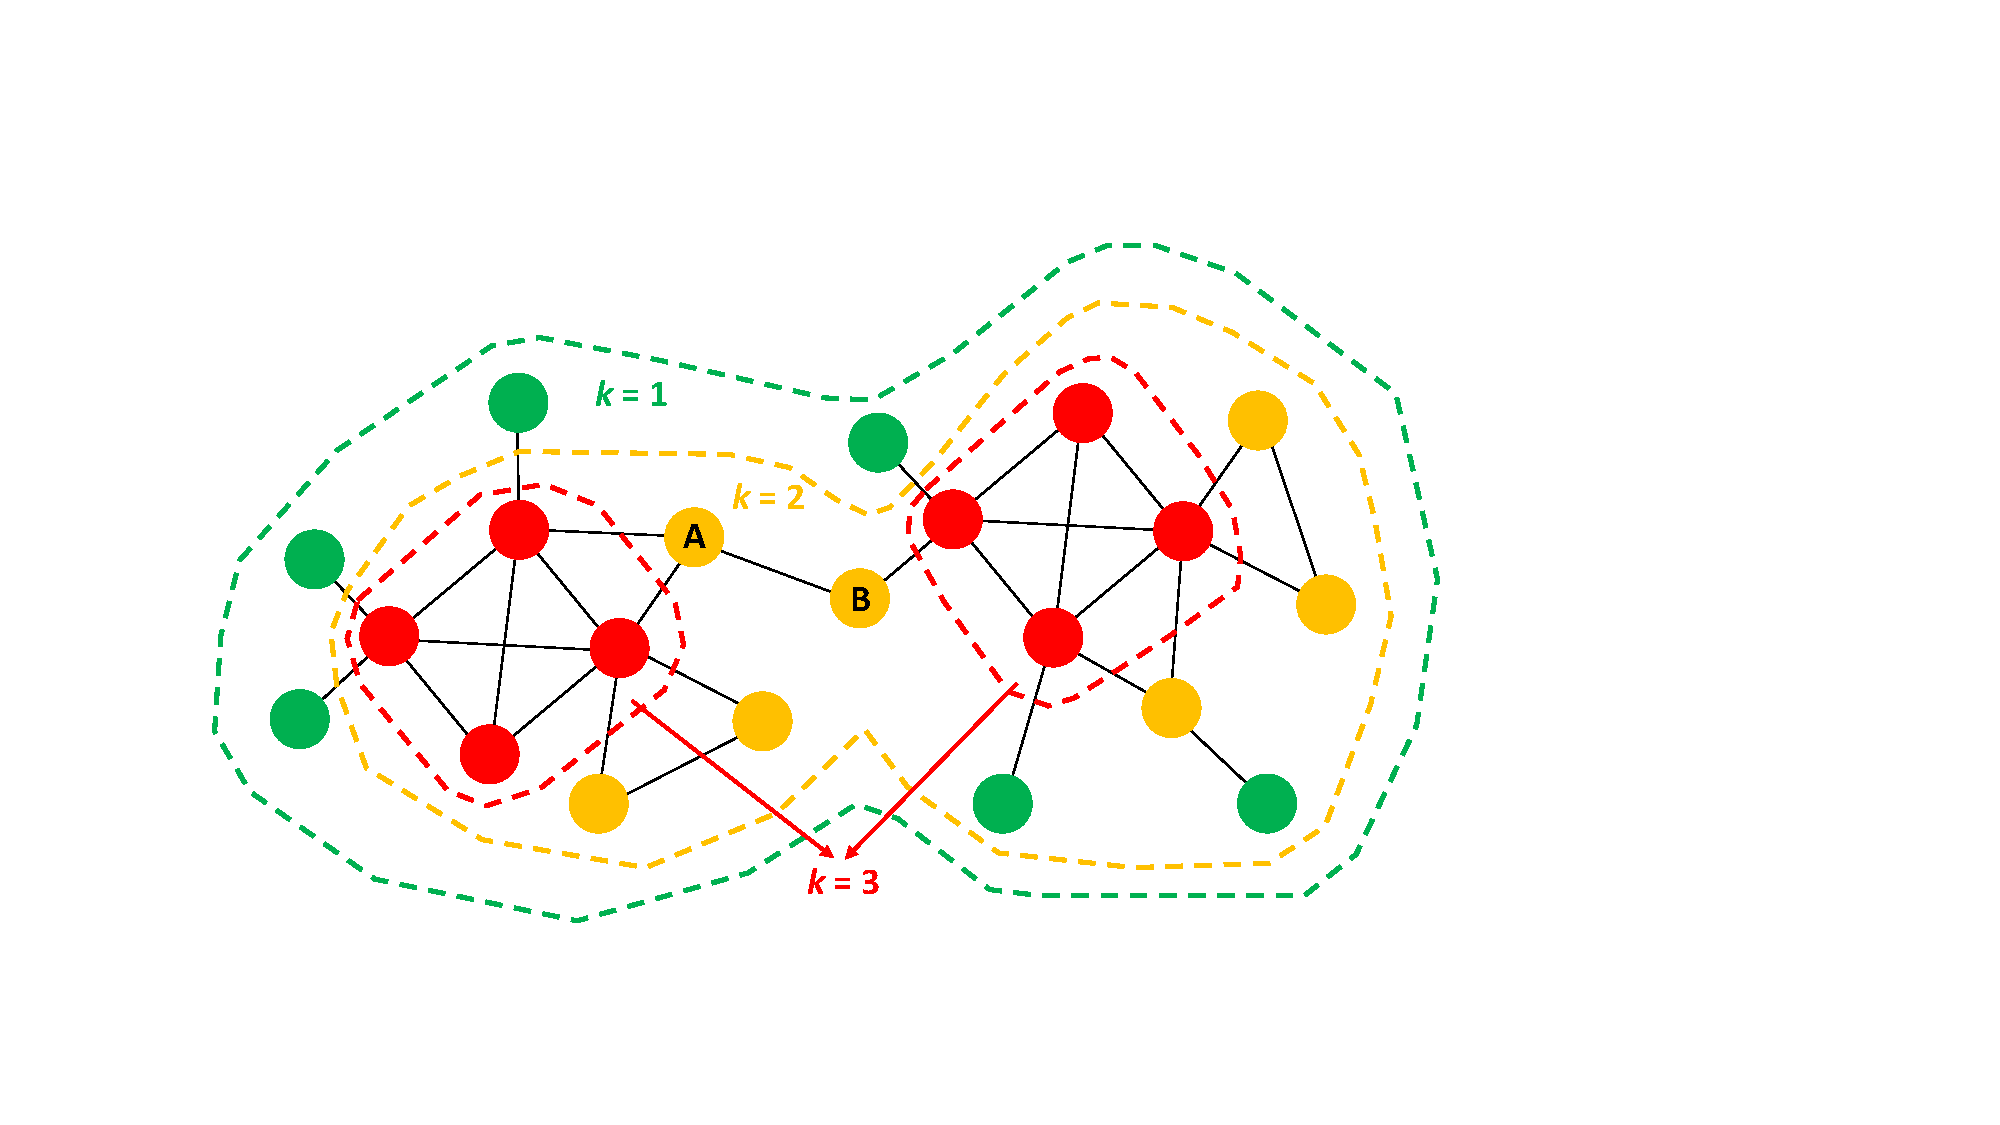
\includegraphics[width=0.8\columnwidth]{kcore_ex}
\vspace{-2mm}
\caption{Illustration of $k$-Cores}\label{kcore_ex}
\vspace{-4mm}
\end{figure}

\vspace{1mm}
\noindent {\bf Degeneracy Ordering.} The $k$-core of a graph $G$ is its largest induced subgraph with minimum (vertex) degree $k$. The degeneracy of $G$, denoted by $D(G)$, is the largest value of $k$ for which a $k$-core exists in $G$. 
%
For example, Figure~\ref{kcore_ex} shows the 1-core, 2-core and 3-core of a graph. 
Specifically, the 2-core contains all yellow and red vertices in the yellow dashed contour, since it is the largest induced subgraph where every vertex has degree $\geq 2$, as any green vertex has degree 1. 
Note that even though vertex~$A$ has degree 3, it is not in 3-core since its neighbor $B$ has degree 2 so cannot be in 3-core, hence $A$ has at most 2 neighbors in 3-core. The operation of $k$-core decomposition finds the core number of every $v\in V$, 
denoted by $core(v)$, which is the largest value of $k$ that $v$ belongs to a $k$-core. 
For example, $core(A)=2$ in Figure~\ref{kcore_ex} since $A$ is in 2-core but not 3-core. 
%
The process of $k$-core decomposition~\cite{seidman1983network} can be computed by a peeling algorithm that repeatedly removes a vertex with the minimum current degree at a time~\cite{bz}. For the graph $G$ in Figure~\ref{kcore_ex}, green vertices will first be removed, followed by yellow ones, and finally the red ones, after which no vertex is remaining so we have $D(G)=3$. Accordingly, the algorithm also generates the degeneracy ordering of vertices in $G$ where green vertices go first, followed by yellow ones and then red ones. 
%
Note that $D(G)$ is a small value in real graphs, since a high-degree vertex tends to appear later in the degeneracy ordering, so many of its neighbors have already been removed by peeling.

\begin{table}[t]
  \caption{M$k$P Algorithms and Their Pruning Techniques~\cite{akhlaque_vldb}}\label{table:mapping}
  \vspace{-3mm}
  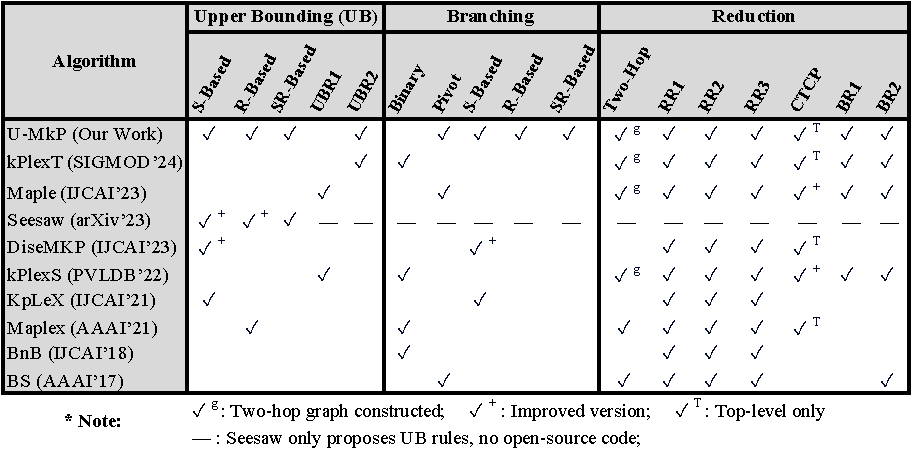
\includegraphics[width=\columnwidth]{mapping-narrow.pdf}
   \vspace{-8mm}
\end{table}

\vspace{1mm}
\noindent {\bf Related Work on M$k$P Algorithms.} Recall from Figure~\ref{fig:dominance} on Page~\pageref{fig:dominance} that many M$k$P algorithms have been proposed in recent years. Earlier works are mainly from the AI community (since it is a search problem) including Maple~\cite{Maple}, Seesaw~\cite{seesaw}, DiseMKP~\cite{DiseMKP}, KpLeX~\cite{KpLeX-MKP}, Maplex~\cite{Maplex}, BnB~\cite{BnB} and BS~\cite{BS}; while more recent works are from the DB community including U-M$k$P~\cite{akhlaque_vldb}, AltRB~\cite{clong_vldb}, kPlexT~\cite{kPlexT} and kPlexS~\cite{kPlexS}. 
%
These M$k$P algorithms have proposed many sophisticated pruning techniques during subgraph exploration that fall in three categories, those for (1)~branching, (2)~bounding, and (3)~reduction. The work of U-M$k$P~\cite{akhlaque_vldb} unifies all techniques into its framework except for new ones proposed by AltRB~\cite{clong_vldb}, as summarized in Table~\ref{table:mapping} (directly from~\cite{akhlaque_vldb}), and please refer to~\cite{akhlaque_vldb} for the detailed statement and proof of each technique. In this paper, we focus on describing those different techniques adopted by U-M$k$P's default configuration (that is tuned to work well in general) and AltRB that really matter for performance (note that some pruning techniques turn out to have negligible impact on real performance), while skipping the common techniques enabled by all the competitive algorithms, such as UBR2 in Table~\ref{table:mapping} that is initially proposed by kPlexT~\cite{kPlexT} and turns out to be so effective that subsequent works U-M$k$P and AltRB adopt it by default.

To achieve good performance consistently, U-M$k$P~\cite{akhlaque_vldb} uses S-based branching method when $k\leq 5$ and pivot-based method when $k>5$. AltRB~\cite{clong_vldb} proposes an alternated reduction-and-bound (abbr.\ altRB) method that significantly reduces the search space and not covered by U-M$k$P. Besides these effective techniques, U-M$k$P and AltRB share a very similar algorithm framework making it easy to unify them, except that (1)~AltRB replaces CTCP with a variant reduction technique called CF-CTCP, and (2)~it replaces the heuristic algorithm originally proposed by kPlexS~\cite{kPlexS} to find an initial large $k$-plex during the preprocessing step with a different heuristic algorithm called KPHeuris. These changes do not show prominent performance improvement on most graphs as shown in the ablation study results from Tables~12-15 in the appendix of~\cite{clong_vldb}.

%toAkhalque: seems CF-CTCP and KPHeuris are reported very effective on some graphs in their paper... we should've integrated them in U-M$k$P as well

\vspace{-1mm}
\section{M$k$P Algorithm Framework and Techniques}\label{sec:kplex}

In this section, we present the algorithm frameworks of U-M$k$P~\cite{akhlaque_vldb} and AltRB~\cite{clong_vldb}, focusing on the branching methods of U-M$k$P and the alternated reduction-and-bound (abbr.\ altRB) method of AltRB.

\vspace{-1mm}
\subsection{A Unified Algorithm Framework}

\begin{figure}[t]
  \includegraphics[width=0.9\columnwidth]{CTCP}
  \vspace{-2mm}
  \caption{Illustration of CTCP}\label{fig:ctcp}
  % \vspace{-4mm}
\end{figure}
\setlength{\textfloatsep}{3pt}

\vspace{1mm}
\noindent{\bf Initial Graph Shrinking \& CTCP.} Algorithm~\ref{algo:toplevel} shows the pseudocode to create top-level search branches $T_{\{v_i\}}$ as {\bf\em adopted by both U-M$k$P and AltRB}, where Line~4 first shrinks the input graph $G$ based on the parameter $k$. Let $P$ be the current largest $k$-plex found, then to find a larger $k$-plex with size at least $|P|+1$, we only need to consider those vertices with degree at least $\tau_v=(|P|+1-k)$ (otherwise, the vertex will miss more than $k$ edges in the larger $k$-plex). Line~4 uses the CTCP (Core-Truss Co-Pruning) reduction method proposed in kPlexS~\cite{kPlexS} that is a tighter version: we only need to consider those vertices with degree at least $\tau_v=(|P|+1-k)$ and those edges $(u, v)$ where $u$ and $v$ share at least $\tau_e=(|P|+1-2k)$ common neighbors (see~\cite{akhlaque_vldb} for the details). Figure~\ref{fig:ctcp} shows an illustration where vertices and edges below thresholds are alternately pruned. AltRB uses a variant called CF-CTCP that further reduces the redundant computations in CTCP. 
%
Since subgraph exploration is conducted on the shrunk $G$ after Line~4, {\bf\em our machine learning model uses input features extracted from the shrunk graph rather than the original input graph that is much larger.}

Besides shrinking the initial graph $G$ in Line~4, CTCP is also called in Line~12 (right after Line~11 removes $v_i$ from $G$), to shrink $G$ further for use by future iterations, since new edges (e.g., $v_i$'s adjacent ones) may have $d_G(u, v)$ reduced below $\tau_e$. By passing $\{v\}$ as the second argument, CTCP can propagate pruning from $v$ and those newly updated edges with $d_G(u, v)<\tau_e$ to minimize its graph update footprint using the method described in~\cite{kPlexS}.

\begin{algorithm}[!t]
    \DontPrintSemicolon
    \KwIn{A graph $G=(V, E)$ and an integer $k\ge 2$}
    \KwOut{A maximum $k$-plex in $G$}
    \SetKwBlock{Begin}{function}{end function}
    \Begin($\text{top\_branching}{(}G{)}$){
        $P, ub \gets $ find\_init($G$)\ \ \ \ \ \# global variables\;\label{top:l1}
        {\bf if} $|P|\ge ub$ {\bf then\ \ return $P$}\;\label{top:l2}
        CTCP($G$, $\emptyset$, $|P|+1-k$, $|P|+1-2k$)\;\label{top:l3}
        Sort $[v_1,\dots, v_n]$ following degeneracy ordering of $G$\;\label{top:l4}
        \For{$i=1$ to $|V|$}{\label{top:l5}
            $H_1 \gets N(v_i) \cap \{v_{i+1}, \dots, v_n\}$\;\label{top:l6}
            $H_2 \gets N(H_1) \cap \{v_{i+1}, \dots, v_n\}$\;\label{top:l7}
            $g \gets$ the subgraph of $G$ induced by $\left(\left\{v_i\right\} \cup H_1\cup H_2\right)$\;\label{top:l8}
            \text{BB}($\{v_i\}, V(g)- \{v_i\}, g$)\ \ \ \ \ \# call a BB variant\;\label{top:l9}
            Remove $v_i$ from $G$\;\label{top:l10}
            CTCP($G$, $\{v_i\}$, $|P|+1-k$, $|P|+1-2k$)\;\label{top:l11}
        }
        \Return{$P$}\;
}
\caption{Top-Level Branching {($c = 2$)}}
\label{algo:toplevel}
\end{algorithm}
\setlength{\textfloatsep}{0pt}

\vspace{1mm}
\noindent{\bf Top-Level Branching \& Top-Level Subgraphs.} In Algorithm~\ref{algo:toplevel}, we assume there are two globally maintained variables accessible any time during subgraph exploration: (1)~$P$: the current largest $k$-plex found, and (2)~$ub$: size upper bound of an M$k$P. 
These two variables are initialized in Line~2 using a heuristic algorithm that finds a large initial $P$ as a preprocessing step; $P$ will also be updated during subgraph exploration whenever a larger $k$-plex is found, so that if we know that a branch cannot generate a $k$-plex larger than $|P|$, it can be pruned without exploration. If $|P|$ equals $ub$, then the initial $P$ is already an M$k$P and is thus returned in Line~3. Otherwise, Line~4 then further prunes $G$ using CTCP.

Recall from Theorem~\ref{lemma::diameter0} that reasonably large $k$-plexes ($|P|> 2k-c$) have diameter $\Delta(P)\leq c$. In other words, for the top-level nodes ${v_i}$ ($v_i=a$, $b$, $c$, $d$) in Figure~\ref{fig:set-enum}, the branch $T_{\{v_i\}}$ under it only needs to consider a subgraph of $G$, denoted by $g_i=(V_i, E_i)$, where vertices are within $c$ hops from $v_i$. We call $g_i$ as the {\bf\em top-level subgraph} of $T_{\{v_i\}}$. 
%
It is worthwhile to shrink $G$ to $g_i$, and explore subgraphs in the branch $T_{\{v_i\}}$ over $g_i$ since (1)~$g_i$ is much smaller than $G$ so checking the neighbors of each vertex becomes much faster, and (2)~this is an efficient one-time processing that can benefit the entire branch $T_{\{v_i\}}$. In contrast, when processing $T_{\{v_i\}}$, even though whenever a vertex $v$ is added to $S$, we can shrink $g_i$ further to remove vertices more than $c$ hops away from $v$, this cost is associated with each expansion of $S$ and so not worthwhile. 

We then create branches $T_{\{v_i\}}$ in the degeneracy ordering as shown in Lines~5-6, which keeps the sizes of all $g_i$'s small to avoid having a giant branch that needs to search a deep set-enumeration subtree with potentially high node fanouts. This is because a high-degree vertex $v_i$ tends to appear later in the degeneracy ordering, so $V_i$ has excluded many neighbors of $v_i$ originally in $V$ (see Line~11). 

Without loss of generality, assume that $c=2$, that is, an M$k$P $P$ has $|P|\ge2k-1$ (i.e., $|P|>2k-2$). 
%
To create $g_i$ for each $v_i$, Line~7 first obtains one-hop neighbors of $v_i$ in $V_i$, and Line~8 then uses them to obtain the two-hop neighbors (where $N(H_1)=\cup_{v\in N(H_1)}N(v)$); finally, Line~9 creates $g_i$ using them (i.e., excluding other vertices in $V_i$ that are $>$ 2 hops away from $v_i$). 
%
{ Note that it is easy to extend $g_i$ for the general case of $c$. For example, when $c=3$, we can additionally compute $H_3 \gets N(H_2) \cap \{v_{i+1}, \dots, v_n\}$ and then compute $g_i$ to be the subgraph of $G$ induced by $\left(\left\{v_i\right\} \cup H_1\cup H_2\cup H_3\right)$.}

Once $g_i$ is created, Line~10 then explores it by extending $S=\{v_i\}$ using branch and bound. For now, we can think of BB(.) simply as BB\_basic(.) presented in Algorithm~\ref{algo:BB}, and two variants will be presented for U-M$k$P and AltRB, respectively. 
%
We then remove $v_i$ from $G$ in Line~11 (similar to Line~5 of Algorithm~\ref{algo:BB}) so that later branches will not consider $v_i$ to avoid redundancy. Note that we do not actually need to do the intersections in Lines~7 and~8 since $\{v_1, \ldots, v_{i-1}\}$ have already been removed in previous iterations.

\begin{algorithm}[!t]
  \DontPrintSemicolon
  \SetKwBlock{Begin}{function}{end function}
  \Begin($\text{reduce\_and\_prune}{(}S, R, g{)}$\ \ // returns if $T_S$ is pruned){ %========= add a comment that return is_pruned
  Apply reduction rules to $(S, R, g)$\ \ // altRB may update $ub$\;
  {\bf if} ($|P|=ub$) {\bf then\ } \Return{true}\;
  %\If{$g$ is a $k$-plex}{
  \If{$g_\text{union}=g[S\cup R]$ is a $k$-plex}{
    {\bf if} $|S|+|R|>|P|$ {\bf then}\ \  $P\gets S\cup R$\;
    \Return{true}\;
  }
  % {\bf if} { seesaw\_UB$(S, R, g) \le |P|$} {\bf then\ } \Return{true}\;
  {\bf if} no candidate in $R$ is valid {\bf then\ } \Return{true}\;
  \Return{false}
}
\caption{Reduction and Pruning Function in AltRB}
\label{algo:reduce-and-prune}
\end{algorithm}
\setlength{\textfloatsep}{0pt}

\vspace{1mm}
\noindent{\bf The Reduction Procedure.} Recall from Line~2 of Algorithm~\ref{algo:BB} that BB(.) first calls reduce\_and\_prune(.) over the instance $(S,R, g)$ for further reduction before extending $S$ with vertices from $R$, the pseudocode of which is shown in Algorithm~\ref{algo:reduce-and-prune}. 
%
Specifically, Line~2 first applies the various reduction rules to reduce the candidate size of $R$. Note that some rules may directly move some candidates in $R$ into $S$, such as {\bf BR1} and {\bf BR2} in U-M$k$P~\cite{akhlaque_vldb}. Also, while $ub$ does not change after the preprocessing stage in U-M$k$P~\cite{akhlaque_vldb}, it may be updated the by altRB method of AltRB~\cite{clong_vldb}. % umkp runs line 2 before line 1 since ub does not change, may be able to avoid line 1's cost


........... here ............... U-M$k$P~\cite{akhlaque_vldb}, AltRB~\cite{clong_vldb}


checks if the current $P$ already reaches the maximum possible size $ub$, and if so, it returns {\em true} to notify BB(.) to terminate its subgraph exploration (see Line~2 of Algorithm~\ref{algo:BB}). 
Right after the call of BB(.) in Line~10 of Algorithm~\ref{algo:toplevel}, we can check if $|P|=ub$ and return $P$ directly if so to terminate early.

Before extending $S$ with vertices in $R$ (e.g., Lines~3--5 in Algorithm~\ref{algo:BB}), we first conduct a look-ahead pruning in Line~4 to see if the entire $g_\text{union}=g[S\cup R]$ is a $k$-plex, and if so, Line~6 returns true so that Line~2 of Algorithm~\ref{algo:BB} will return directly to terminate its exploration of $T_S$. Moreover, if $S\cup R$ is larger than the current $P$, $P$ is updated with $S\cup R$ in Line~5.

Finally, we check if $T_{S}$ can still produce a $k$-plex larger than $P$, and if not, Line~7 returns {\em true} to let BB(.) terminate its exploration of $T_S$. The function partition(.) (to be introduced in Section~\ref{sec:branch}) uses upper-bound-based pruning to return the subset of vertices in $R$, denoted by $B$, that is still worth branching with (i.e., to extend $S$ only with a vertex in $B$ in the next step), and if $B=\emptyset$, there is nothing worth extending with so the entire $T_S$ is pruned.

... line 2 and line 7 differ;

%\noindent{\bf Reduction and Upper-Bound-Based Branch Pruning.}

\vspace{-1mm}
\section{Set Representations}\label{sec:set}

\vspace{-1mm}
\section{Learning-Based Algorithm Selection}\label{sec:learn}

... First summarize algorithm candidates here ...

\vspace{-1mm}
\section{Experiments}\label{sec:results}

\vspace{-1mm}
\section{Conclusion}\label{sec:conclude}

\bibliographystyle{ACM-Reference-Format}
\bibliography{references}

\end{document}
